\subsection{Case Study on Two Production Server Applications}
Using basic blocks extracted from two production applications in Google---Spanner~\cite{spanner} and Dremel~\cite{dremel},
we additionally validated the performance models discussed in this paper 
(except OSACA, due to licensing issues).
Spanner is a highly available, globally distributed database,
designed to scale up to millions of machines and trillions of database rows \cite{spanner}.
Dremel is a scalable,
interactive ad-hoc query system for analysis of read-only data,
capable of running aggregation queries over trillion-row tables in seconds \cite{dremel}.

We show the composition of basic blocks these two applications in Figure~\ref{fig:google-blocks}.
Spanner and Dremel spend almost half of the time executing load instructions (category-6)---40\% and 50\%, respectively. 
Compared to similar applications from our 
data set,
they spend significantly more
time---12\% and 9\%, respectively---executing vectorized basic blocks.
The closest applications in our dataset are
SQLite and Redis, and in contrast, they spend 5.0\% and 0.2\%
of the time executing (partially) vectorized basic blocks (category-1 and -2).
This is evidence of Google's effort to optimize
these applications.

\begin{figure}[htbp!]
    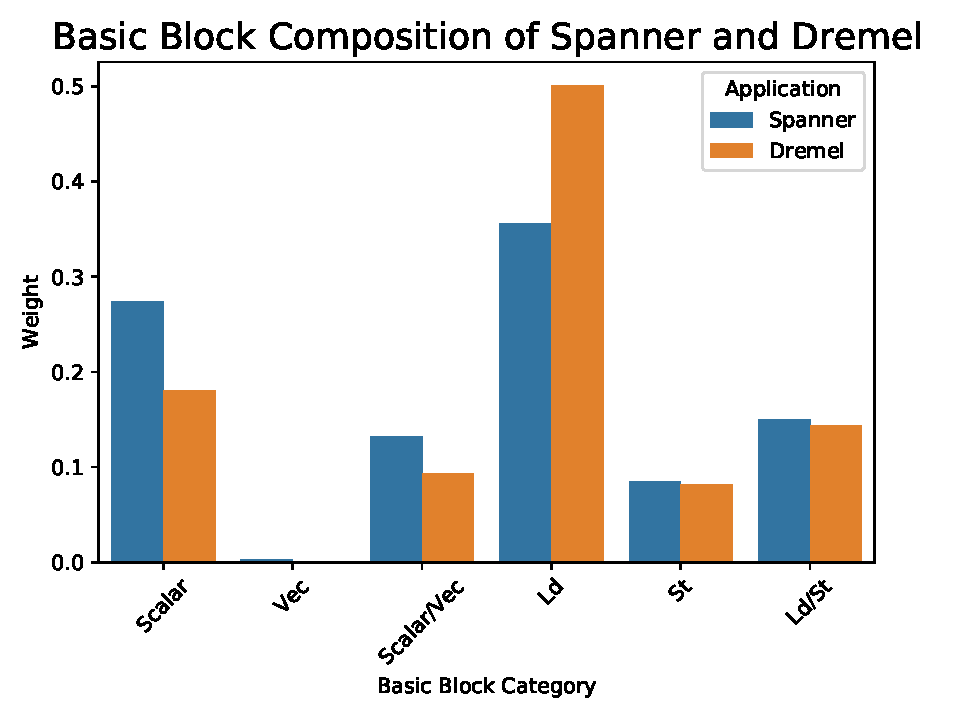
\includegraphics[width=0.95\columnwidth]{figures/google-blocks.pdf}
    \caption{Basic Block composition of Spanner. Each basic block is weighted by its
    execution frequency.}
    \label{fig:google-blocks}
\end{figure}

On a Haswell machine, we use our profilers
to measure the throughput of the 100,000 most frequently executed  basic blocks
from the two applications. Table~\ref{tab:google-numbers} shows the accuracy
of IACA, llvm-mca, and Ithemal predicting these basic blocks.
Given the dominant basic block categories of the 
two applications,
their predictions are consistent with our previous analysis,
with one exception:
llvm-mca, which has an average prediction error of 25\% on Haswell, predicts noticeably better
when processing Spanner's and Dremel's basic blocks.

\begin{table}[h]
\begin{tabular}
{|p{0.15\columnwidth}|p{0.15\columnwidth}|p{0.15\columnwidth}|p{0.15\columnwidth}|p{0.15\columnwidth}|}
\hline

\textbf{Application} & \textbf{Model} &
\textbf{Average Error} & \textbf{Weighted Error} & \textbf{Kendall's Tau Coefficient} \\
\hline

Spanner & IACA & 0.1892 & 0.1659 & 0.7786\\
    & llvm-mca & 0.1764 & 0.1519 & 0.7623\\
    & Ithemal & \textbf{0.1629} & \textbf{0.1414} & \textbf{0.7799}\\
\hline

Dremel & IACA & 0.1883 & 0.1846 & 0.7835\\
    & llvm-mca & 0.1777 & \textbf{0.1831} & 0.7685\\
    & Ithemal & \textbf{0.1640} & 0.1871 & \textbf{0.7862}\\

\hline
\end{tabular}
\\
\caption{Accuracy of IACA, llvm-mca, and Ithemal predicting basic blocks from Spanner and Dremel.
Bolded entries are the best among the three evaluated models.
Kendall's tau coefficient~\cite{kendalltau}
measures the fraction of pairwise throughput ordering preserved by a given model;
so the higher the better.
The ``Weighted Error'' column shows prediction errors weighted by a basic block's runtime frequency.}
\label{tab:google-numbers}
\end{table}